% ****** Start of file apssamp.tex ******
%
%   This file is part of the APS files in the REVTeX 4.2 distribution.
%   Version 4.2a of REVTeX, December 2014
%
%   Copyright (c) 2014 The American Physical Society.
%
%   See the REVTeX 4 README file for restrictions and more information.
%
% TeX'ing this file requires that you have AMS-LaTeX 2.0 installed
% as well as the rest of the prerequisites for REVTeX 4.2
%
% See the REVTeX 4 README file
% It also requires running BibTeX. The commands are as follows:
%
%  1)  latex apssamp.tex
%  2)  bibtex apssamp
%  3)  latex apssamp.tex
%  4)  latex apssamp.tex
%
\documentclass[superscriptaddress,unsortedaddress,
%runinaddress,
%frontmatterverbose, 
%preprint,
%preprintnumbers,
%nofootinbib,
%nobibnotes,
%bibnotes,
 amsmath,amssymb,
 aps,
%pra,
%prb,
%rmp,
%prstab,
%prstper,
%floatfix,
]{revtex4-2}

\usepackage{amsmath}
\usepackage{amsthm}
\usepackage{amssymb}
\usepackage[top=4cm,bottom=4cm,left=2.8cm,right=3.75cm,asymmetric,twoside]{geometry}
\usepackage{graphicx}
\usepackage{fancyhdr}
\usepackage{comment}
\usepackage{tikzorbital}
\usepackage{array} % center tables + 2 next lines
\newcolumntype{P}[1]{>{\centering\arraybackslash}p{#1}}
\newcolumntype{M}[1]{>{\centering\arraybackslash}m{#1}}
\usepackage{multirow} % confusion matrix
\newcommand\MyBox[2]{
  \fbox{\lower0.75cm
    \vbox to 2.0cm{\vfil
      \hbox to 2.0cm{\hfil\parbox{1.4cm}{#1\\#2}\hfil}
      \vfil}%
  }%
}
\usepackage{grffile}
\usepackage{epigraph} % quote
\usepackage{wrapfig} %wrapping text to fig
\usepackage{tikz} %draw figures

\usepackage{subcaption} %subcaption
\usepackage[font=small,labelfont=bf,width=0.9\textwidth]{caption}
\captionsetup[table]{skip=10pt}
\usepackage[T1]{fontenc}
\usepackage[sc, osf]{mathpazo}
\usepackage[euler-digits]{eulervm}
\usepackage{booktabs}
\usepackage{enumerate}
\usepackage{commath}
\usepackage{mathtools}
\usepackage[utf8]{inputenc}
\usepackage{pgfplots}
\usepgfplotslibrary{groupplots,dateplot}
\usetikzlibrary{patterns,shapes.arrows, arrows.meta,bending, shapes,calc,fadings,decorations.pathreplacing,positioning,arrows.meta}
\pgfplotsset{compat=newest}

\usepackage{sansmath}
\tikzset{>=stealth,
OptimumStyle/.style={align=center,anchor=east,rotate=90,font=\scriptsize}
}
\pgfplotsset{%samples=101,
axis lines = left,
every axis plot/.append style={line width=2pt},
}
% Include font for the identity operator
\usepackage{dsfont}
\usepackage[binary-units=true]{siunitx}
\usepackage{makecell}
\usepackage{longtable}
\usepackage{dcolumn}% Align table columns on decimal point
\usepackage{bm}% bold math
\usepackage{physics}
\usepackage{lipsum}
\usepackage{siunitx}
\usepackage{color}
\sisetup{separate-uncertainty}

\usepackage{forest}
\forestset{
    .style={
        for tree={
            base=bottom,
            child anchor=north,
            align=center,
            s sep+=1cm,
    straight edge/.style={
        edge path={\noexpand\path[\forestoption{edge},thick,-{Latex}]
        (!u.parent anchor) -- (.child anchor);}
    },
    if n children={0}
        {tier=word, draw, thick, rectangle}
        {draw, diamond, thick, aspect=2},
    if n=1{%
        edge path={\noexpand\path[\forestoption{edge},thick,-{Latex}]
        (!u.parent anchor) -| (.child anchor) node[pos=.2, above] {Y};}
        }{
        edge path={\noexpand\path[\forestoption{edge},thick,-{Latex}]
        (!u.parent anchor) -| (.child anchor) node[pos=.2, above] {N};}
        }
        }
    }
}
\tikzset{
  green arrow/.style={
    midway,green,sloped,fill, minimum height=2cm, single arrow, single arrow head extend=.5cm, single arrow head indent=.25cm,xscale=0.3,yscale=0.15,
    allow upside down
  },
  yellow arrow/.style={
    midway,yellow,sloped,fill, minimum height=2cm, single arrow, single arrow head extend=.5cm, single arrow head indent=.25cm,xscale=0.3,yscale=0.15,
    allow upside down
  },
  black arrow/.style 2 args={-stealth, shorten >=#1, shorten <=#2},
  black arrow/.default={1mm}{1mm},
  tree box/.style={draw, rounded corners, inner sep=1em},
  node box/.style={white, draw=white, text=black, rectangle, rounded corners},
}


\newcommand{\oliver}[1]{\textcolor{violet}{#1}} 
\newcommand{\morten}[1]{\textcolor{green}{#1}}
\newcommand{\sebastian}[1]{\textcolor{cyan}{#1}}
\newcommand{\marianne}[1]{\textcolor{blue}{#1}}
\newcommand{\oyvind}[1]{\textcolor{maroon}{#1}}
\newcommand{\lasse}[1]{\textcolor{red}{#1}}

\begin{document}

\title{Supplementary Material \\ 
%Predicting Solid State Qubit Candidates}
Predicting Solid State Material Platforms for Quantum Technologies}


\author{Oliver Lerst{\o}l Hebnes}
\affiliation{Your new job} 
\affiliation{Department of Physics and Center for Computing in Science Education, University of Oslo, N-0316 Oslo, Norway}

\author{Marianne Etzelm\"uller Bathen}
\affiliation{Advanced Power Semiconductor Laboratory, ETH Zürich, 8092  Zürich,  Switzerland}
\affiliation{Department of Physics and Center for Materials Science and Nanotechnology, University of Oslo, N-0316 Oslo, Norway}

\author{{\O}yvind Sigmundson Sch{\o}yen}
\affiliation{Department of Physics and Center for Computing in Science Education, University of Oslo, N-0316 Oslo, Norway}

\author{Sebastian G. Winther-Larsen}
\affiliation{Menon Economics, N-0369 Oslo, Norway}
\affiliation{Department of Physics and Center for Computing in Science Education, University of Oslo, N-0316 Oslo, Norway}

\author{Lasse Vines}
\affiliation{Department of Physics and Center for Materials Science and Nanotechnology, University of Oslo, N-0316 Oslo, Norway}

\author{Morten Hjorth-Jensen}
\affiliation{Department of Physics and Astronomy and Facility for Rare Ion Beams, Michigan State University, East Lansing, MI 48824, USA}
\affiliation{Department of Physics and Center for Computing in Science Education, University of Oslo, N-0316 Oslo, Norway}

\pacs{02.70.Ss, 31.15.A-, 31.15.bw, 71.15.-m, 73.21.La}

\maketitle


\noindent \textbf{Contents:} 
\begin{itemize}
    \item \textit{Supplementary methods.} \\   Additional information on the featurization process and optimization of the machine learning models. 
    \item \textit{Supplementary results.} \\  Statistics and tables over the materials that were predicted by the machine learning models based on the training sets derived using the three different data mining approaches. 
    \item \textit{Supplementary references.}  
\end{itemize}

\newpage 

\section*{Supplementary methods}
\subsection*{Featurization}
To apply Matminer's featurization tools, we extend an existing implementation by \citeauthor{Breuck2021} \cite{Breuck2021}. 
Table~\ref{table:featurizers} contains an overview of this work's chosen 39 featurizers from Matminer. The featurization process results in $4876$ descriptors. 

The motivation behind the choice of featurizers is that we do not precisely know which features describe a suitable potential host. Therefore, we strive to collect an achievable quantity of descriptors with the hope of getting wiser in terms of prediction potential materials for quantum technologies. 


\begin{center}
\begin{longtable}{M{3.5cm} M{6.5cm} M{2.0cm}}
\caption{Descriptions of the 39 featurizers from Matminer that have been emplyed in this work. Descriptions are either found from Ref. \cite{Ward2018} or from the project's Github page. For entries lacking references, we refer to Ref.~\cite{Ward2018}.}
\label{table:featurizers} 
\\ \hline
Features & Description & Reference \\
\hline 
  \textbf{Composition features} & & \\ 
  AtomicOrbitals & Highest occupied molecular orbital (HOMO) & \cite{Kotochigova1997}  \\   
   & and lowest unoccupied molecular orbital (LUMO) &  \\   
  AtomicPacking-Efficiency & Packing efficiency & \cite{Laws2015}  \\   
  BandCenter & Estimate absolute position of band center  & \cite{Butler1978} \\   
   & using geometric mean of electronegativity &  \\  
  ElementFraction & Fraction of each element in a composition &    \\   
  ElementProperty & Statistics of various element properties & \cite{Ong2013,Ward2016, Deml2016}  \\   
  IonProperty & Maximum and average ionic character & \cite{Ward2016} \\   
  Miedema & Formation enthalpies of intermetallic compounds, solid solutions, & \cite{Weeber1987} \\   
   & and amorphous phases using semi-empirical Miedema model &  \\   
  Stoichiometry & $L^p$ norm-based stoichiometric attributes & \cite{Ward2016} \\   
  TMetalFraction & Fraction of magnetic transition metals & \cite{Deml2016}  \\   
  ValenceOrbital & Valence orbital attributes such as & \cite{Ward2016}  \\   
   &  the mean number of electrons in each shell &   \\   
  YangSolid-Solution & Mixing thermochemistry and size mismatch terms & \cite{Yang2012} \\
    \hline 
  \textbf{Oxide composition features} &  &  \\
  Electronegativity-Diff & Statistics on electronegativity difference & \cite{Deml2016} \\   
   &  between anions and cations & \\ 
  OxidationStates & Statistics of oxidation states & \cite{Deml2016}  \\   
\hline 
  \textbf{Structure features} & & \\   
  DensityFeatures & Calculate density, volume per atom and packing fraction & - \\   
  GlobalSymmetry-Features & Determines spacegroup number, crystal system  & - \\   
   & (1-7) and inversion symmetry & \\ 
  RadialDistribution-Function & Calculates the radial distribution  & - \\   
   & function of a crystal system & \\ 
  CoulombMatrix & Generate the Coulomb matrix for nuclear interactions  & \cite{Rupp2012}  \\    
  %CoulombMatrix & Generate the Coulomb matrix, which is a representation of the nuclear coulombic interaction of the input structure. & \cite{Rupp2012}  \\      
  PartialRadial-Distribution-Function & Compute the partial radial distribution  & \cite{Schuett2014}  \\   
   & function of a crystal structure & \\ 
  SineCoulomb-Matrix & Computes a variant of the coulomb matrix & \cite{Faber2015}  \\   
   & developed for periodic crystals & \\ 
  EwaldEnergy & Computes the energy from Coulombic interactions  & \cite{Ewald1921}  \\   
   & based on charge states of each site & \\ 
  BondFractions & Compute the fraction of each bond in a  & \cite{Hansen2015}  \\   
   & structure, based on nearest neighbors & \\ 
  Structural Heterogeneity & Calculates the variance in bond lengths and  & \cite{Ward2017}  \\   
   & atomic volumes in a structure & \\ 
  MaximumPacking-Efficiency & Calculates the maximum packing efficiency of a structure & \cite{Ward2017} \\   
  Chemical-Ordering & Computes how much the ordering of species  & \cite{Ward2017}  \\   
   & differs from random in a structure & \\ 
  XRDPowder-Pattern & 1D array representing normalized powder diffraction & \cite{Ong2013} \\ 
   &of a structure as calculated by pymatgen  & \\ 
    \hline 
  \textbf{Site features} & & \\
  AGNI-Fingerprints & Calculates the product integral of RDF & \cite{Botu2014}  \\    
   & and Gaussian window function  & \\ 
  AverageBond- Agle & Determines the average bond angle of a specific  & \cite{Jong2016}  \\
   & site with its nearest neighbors  & \\ 
  AverageBond-Length & Determines the average bond length between one specific site & \cite{Jong2016}  \\ 
   & and all its nearest neighbors  & \\ 
  BondOrientational-Parameter & Calculates the averages of spherical  & \cite{Seko2017, Steinhardt1983}  \\ 
   & harmonics of local neighbors & \\ 
  ChemEnvSite-Fingerprint & Calculates the resemblance of given sites to ideal & \cite{Waroquiers2017, Zimmermann2017}  \\   
   & environment using pymatgens ChemEnv package  & \\ 
  Coordination-Number & The number of first nearest neighbors of a site & \cite{Zimmermann2017}  \\
  CrystalNN-Fingerprint & A local order parameter fingerprint for periodic crystals & -  \\   
  GaussianSymm-Func & Calculates the gaussian radial and angular symmetry functions  & \cite{Behler2011,Khorshidi2016}  \\   
   & originally suggested for fitting machine learning potentials &  \\ 
  GeneralizedRadial-Distribution-Function & Computes the general radial distribution function for a site & \cite{Seko2017}  \\   
  LocalProperty-Difference & Computes the difference in elemental properties  & \cite{Ward2017, Jong2016} \\   
   & between a site and its neighboring sites & \\ 
  OPSite-Fingerprint & Computes the local structure order parameters & \cite{Zimmermann2017} \\   
   & from a site's neighbor environment  & \\ 
  Voronoi-Fingerprint & Calculates the Voronoi tessellation-based  & \cite{Peng2011,Wang2019} \\
   & features around a target site & \\ 
\hline     
  \textbf{Density of state features} & & \\
  DOSFeaturizer & Computes top contributors to the density of  & \cite{Dylla2020} \\ 
  & states at the VBM and CBM  & \\ 
  %DOSFeaturizer & Computes top contributors to the density of states at the valence and conduction band edges. Thus includes chemical species, orbital character, and orbital location information. & \cite{Dylla2020} \\
  \hline  
  \textbf{Band structure features} & & \\
  BandFeaturizer & Converts a complex electronic band  & - \\ 
   &structure into discrete quantities  & \\ 
%BandFeaturizer & Converts a complex electronic band structure into quantities such as band gap and the norm of k point coordinates at which the conduction band minimum and valence band maximum occur. & - \\
\hline 
\end{longtable}
\end{center}


\subsection*{Optimization of machine learning models}

In the evaluation of the machine learning models for the three different approaches, we apply a $5\times 5$ stratified cross-validation when searching for the optimal hyperparameter combinations. Due to imbalanced training data, we apply four different evaluation metrics to each of the four algorithms for each approach. 

The implementation of the machine learning models was done through the open library of Scikit-learn. By adjusting the majority of the hyperparameters in Sciki-learn, we experienced severe overfitting for random forest, gradient boosting, and decision trees. Therefore, most parameters are the default values defined by Scikit-learn. The only parameter that we found that could potentially improve the evaluation metric F$1$ was the maximum number of depth for the trees grown, which we adjusted between $1$ and $8$. For logistic regression, we chose to adjust the regularization strength with seven logarithmic adjusted values from $10^{-3}$ to $10^{5}$, and use either $200$ or $400$ iterations to reach convergence. 

When searching for the optimal number of principal components, we iterated over every odd number of principal components from $1$ to the upper restricted number which defines an accumulated variance of $95 \ \%$ from the principal component analysis. Due to a large number of principal components, we end up fitting $25$ folds for each of the $1232$ parameter combinations, totaling up to $30.800$ individual models, just for one arbitrary machine learning algorithm like logistic regression. 

\subsubsection*{Ferrenti approach}
%Ferrenti 
The grid search for the optimal number of principal components for the Ferrenti approach is visualized in Figure~\ref{fig:01-pca}, where we present the mean accuracy on the training set, and the balanced accuracy, precision, recall, and F$1$-score on the test set as a function of principal components used in the models. For each principal component, the optimal combination of hyperparameters based on the F$1$-score is visualized. 

\begin{figure}[ht!]
\begin{subfigure}[b]{1.0\textwidth}
    \centering
    % This file was created by tikzplotlib v0.9.8.
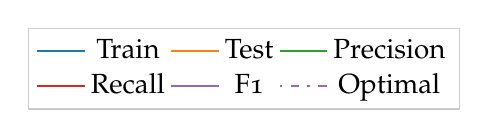
\begin{tikzpicture}

\definecolor{color0}{rgb}{0.12156862745098,0.466666666666667,0.705882352941177}
\definecolor{color1}{rgb}{1,0.498039215686275,0.0549019607843137}
\definecolor{color2}{rgb}{0.172549019607843,0.627450980392157,0.172549019607843}
\definecolor{color3}{rgb}{0.83921568627451,0.152941176470588,0.156862745098039}
\definecolor{color4}{rgb}{0.580392156862745,0.403921568627451,0.741176470588235}
\begin{axis}[%
 hide axis,
 xmin=10,
 xmax=50,
 ymin=0,
 ymax=0.4,
 legend columns=3,
 legend style={
   fill opacity=1,
   draw opacity=1,
   text opacity=1,
   align=center,
   anchor=north,
   draw=white!80!black
 },
 ]
 \addlegendimage{semithick, color0}
 \addlegendentry{Train};
 \addlegendimage{semithick, color1}
 \addlegendentry{Test};
 \addlegendimage{semithick, color2}
 \addlegendentry{Precision};
 \addlegendimage{semithick, color3}
 \addlegendentry{Recall};
 \addlegendimage{semithick, color4}
 \addlegendentry{F1};
 \addlegendimage{semithick, color4, dash pattern=on 1pt off 3pt on 3pt off 3pt}
 \addlegendentry{Optimal};
 \end{axis}

\end{tikzpicture}

  \end{subfigure}
  \par\bigskip
  \begin{subfigure}[b]{0.5\textwidth}
    \input{figures/optimizing-parameters/01-ferrenti-approach-176-LOG}
    \caption{}
    \label{fig:q1-LOG}
  \end{subfigure}%
    \hfill
  \begin{subfigure}[b]{0.5\textwidth}
    \input{figures/optimizing-parameters/01-ferrenti-approach-176-DT}
    \caption{}
    \label{fig:q1-DT}
  \end{subfigure}
  \begin{subfigure}[b]{0.5\textwidth}
    \input{figures/optimizing-parameters/01-ferrenti-approach-176-RF.tex}
    \caption{}
    \label{fig:q1-RF}
  \end{subfigure}%
   \hfill
  \begin{subfigure}[b]{0.5\textwidth}
    \input{figures/optimizing-parameters/01-ferrenti-approach-176-GB.tex}
    \caption{}
    \label{fig:q1-GB}
  \end{subfigure}
  \caption{Four figures displaying hyperparameter search for the Ferrenti approach. The best estimator is visualized for all hyperparameters as a function of principal components during a grid search with a $5\times5$ stratified cross-validation, and the dotted lines mark the optimal hyperparameter-combination. Train stands for normal training accuracy, while test is the balanced accuracy on the test set. Precision, recall, and F$1$ scores are based on the test set. The number of principal components that explain the $95 \ \%$ accumulated variance is $144$, while the optimal model is found using the F$1$-score.}
  \label{fig:01-pca}
\end{figure}

\begin{table}[t]
\centering
\caption{Optimal number of principal components and the respective scores (standard deviation) for each of the four ML models logistic regression (LOG), decision trees (DT), random forests (RF) and gradient boosting (GB) in the Ferrenti approach, as visualized by the dash-dotted line in Figure~\ref{fig:01-pca}.}
\label{tab:01-pc}
\noindent\makebox[\textwidth]{
\begin{tabular}{M{1.0cm} M{1.0cm} M{2.0cm} M{2.0cm}M{2.0cm}M{2.0cm} }
  \hline
  \hline
   Model & PC & Mean test &  Mean precision & Mean recall & mean F1\\
  \hline
  LOG & $171$ & $0.98(0.012)$ & $0.98(0.011)$ & $0.99(0.007)$ & $0.99(0.007)$ \\
  DT & $37$   & $0.77(0.034)$ & $0.84(0.034)$ & $0.85(0.044)$ & $0.84(0.022)$ \\
  RF & $53$   & $0.87(0.027)$ & $0.88(0.022)$ & $0.98(0.010)$ & $0.93(0.014)$ \\
  GB & $107$  & $0.92(0.016)$ & $0.92(0.015)$ & $0.98(0.010)$ & $0.95(0.009)$ \\
  \hline
\end{tabular}
}
\end{table}

In Table~\ref{tab:01-pc}, we include the precise measurements for each of the evaluation metrics for the optimal number of principal components, which is visualized as dotted lines in Fig.~\ref{fig:01-pca}. The relevant hyperparameters for logistic regression were the maximum iterations, which was set at $400$, and the regularization term, which was found optimal at $0.46$. For random forests and decision trees, we find the maximum depth of $7$, while being $4$ for gradient boosting. We find the best performing model is logistic regression, but this model is dependent on a large number of principal components. 

In Figure~\ref{fig:01-fi}, we visualize how the models interpret the principal components that are sorted in descending order by the explained variance, found through a $5\times 5$ stratified cross-validation. To reach the $95 \ \%$ accumulated explained variance, a total of $144$ principal components needs to be involved. We have visualized the first $25$ since this captures the most important information, and we note that most of the important features are found within the first five principal components.

\begin{figure}[ht!]
  \begin{subfigure}[b]{0.5\textwidth}
    \centering
    \input{figures/feature-importance/01-ferrenti-approachLOG-final.tex}
    \label{fig:01-fi-a}
  \end{subfigure}%

  \begin{subfigure}[b]{0.5\textwidth}
    \centering
    \input{figures/feature-importance/01-ferrenti-approachDT-final.tex}
    \label{fig:01-fi-b}
  \end{subfigure}%

  \begin{subfigure}[b]{0.5\textwidth}
    \centering
    \input{figures/feature-importance/01-ferrenti-approachRF-final.tex}
    \label{fig:01-fi-c}
  \end{subfigure}%

  \begin{subfigure}[b]{0.5\textwidth}
    \centering
    \input{figures/feature-importance/01-ferrenti-approachGB-final.tex}
    \label{fig:01-fi-d}
  \end{subfigure}%

  \begin{subfigure}[b]{0.5\textwidth}
    \centering
    % This file was created by tikzplotlib v0.9.8.
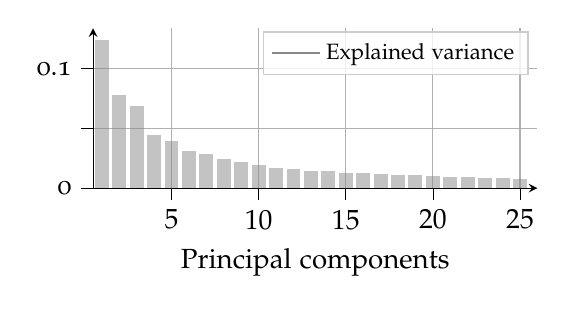
\begin{tikzpicture}

\definecolor{color0}{rgb}{0.8,0.4,0.466666666666667}

\begin{axis}[
height=1.4222438079424382in,
legend style={fill opacity=0.8, draw opacity=1, text opacity=1, draw=white!80!black},
tick align=outside,
tick pos=left,
width=2.8444876158848764in,
x grid style={white!69.0196078431373!black},
xlabel={Principal components},
xmajorgrids,
xmin=0.5, xmax=26,
xtick style={color=black},
y grid style={white!69.0196078431373!black},
ymajorgrids,
ymin=0, ymax=0.133808014644924,
ytick style={color=black},
yticklabels={, 0, , 0.1},
legend style={font=\footnotesize},
]
\draw[draw=none,fill=white!53.3333333333333!black,fill opacity=0.5] (axis cs:0.6,0) rectangle (axis cs:1.4,0.123808014644924);
\draw[draw=none,fill=white!53.3333333333333!black,fill opacity=0.5] (axis cs:1.6,0) rectangle (axis cs:2.4,0.0779020383908885);
\draw[draw=none,fill=white!53.3333333333333!black,fill opacity=0.5] (axis cs:2.6,0) rectangle (axis cs:3.4,0.0690715494994265);
\draw[draw=none,fill=white!53.3333333333333!black,fill opacity=0.5] (axis cs:3.6,0) rectangle (axis cs:4.4,0.0448634890553009);
\draw[draw=none,fill=white!53.3333333333333!black,fill opacity=0.5] (axis cs:4.6,0) rectangle (axis cs:5.4,0.0396017649392185);
\draw[draw=none,fill=white!53.3333333333333!black,fill opacity=0.5] (axis cs:5.6,0) rectangle (axis cs:6.4,0.0309892340254588);
\draw[draw=none,fill=white!53.3333333333333!black,fill opacity=0.5] (axis cs:6.6,0) rectangle (axis cs:7.4,0.0286471759268761);
\draw[draw=none,fill=white!53.3333333333333!black,fill opacity=0.5] (axis cs:7.6,0) rectangle (axis cs:8.4,0.0241373022722755);
\draw[draw=none,fill=white!53.3333333333333!black,fill opacity=0.5] (axis cs:8.6,0) rectangle (axis cs:9.4,0.0219387724823991);
\draw[draw=none,fill=white!53.3333333333333!black,fill opacity=0.5] (axis cs:9.6,0) rectangle (axis cs:10.4,0.0191941500093896);
\draw[draw=none,fill=white!53.3333333333333!black,fill opacity=0.5] (axis cs:10.6,0) rectangle (axis cs:11.4,0.0170987447716404);
\draw[draw=none,fill=white!53.3333333333333!black,fill opacity=0.5] (axis cs:11.6,0) rectangle (axis cs:12.4,0.0163324377943715);
\draw[draw=none,fill=white!53.3333333333333!black,fill opacity=0.5] (axis cs:12.6,0) rectangle (axis cs:13.4,0.0142479118996461);
\draw[draw=none,fill=white!53.3333333333333!black,fill opacity=0.5] (axis cs:13.6,0) rectangle (axis cs:14.4,0.0139471831901937);
\draw[draw=none,fill=white!53.3333333333333!black,fill opacity=0.5] (axis cs:14.6,0) rectangle (axis cs:15.4,0.0125561362477749);
\draw[draw=none,fill=white!53.3333333333333!black,fill opacity=0.5] (axis cs:15.6,0) rectangle (axis cs:16.4,0.0122752355665442);
\draw[draw=none,fill=white!53.3333333333333!black,fill opacity=0.5] (axis cs:16.6,0) rectangle (axis cs:17.4,0.0117377683648439);
\draw[draw=none,fill=white!53.3333333333333!black,fill opacity=0.5] (axis cs:17.6,0) rectangle (axis cs:18.4,0.0108124054147357);
\draw[draw=none,fill=white!53.3333333333333!black,fill opacity=0.5] (axis cs:18.6,0) rectangle (axis cs:19.4,0.0105912984624588);
\draw[draw=none,fill=white!53.3333333333333!black,fill opacity=0.5] (axis cs:19.6,0) rectangle (axis cs:20.4,0.00987028371434172);
\draw[draw=none,fill=white!53.3333333333333!black,fill opacity=0.5] (axis cs:20.6,0) rectangle (axis cs:21.4,0.00946157777094173);
\draw[draw=none,fill=white!53.3333333333333!black,fill opacity=0.5] (axis cs:21.6,0) rectangle (axis cs:22.4,0.00932051055389097);
\draw[draw=none,fill=white!53.3333333333333!black,fill opacity=0.5] (axis cs:22.6,0) rectangle (axis cs:23.4,0.00851928669553865);
\draw[draw=none,fill=white!53.3333333333333!black,fill opacity=0.5] (axis cs:23.6,0) rectangle (axis cs:24.4,0.00821174057436937);
\draw[draw=none,fill=white!53.3333333333333!black,fill opacity=0.5] (axis cs:24.6,0) rectangle (axis cs:25.4,0.00796122578616887);
\addlegendimage{semithick, color=white!53.3333333333333!black};
\addlegendentry{Explained variance};
\end{axis}

\end{tikzpicture}

    \label{fig:01-fi-e}
  \end{subfigure}%

  \caption{Five figures visualizing different parameters for the $25$ most principal components ranked in descending order by the explained variance for the Ferrenti approach. The panels show the logistic regression coefficients, decision trees feature importance, random forests feature importance, gradient boosting feature importance, and explained variance that is retained by choosing each of the eigenvectors. }
  \label{fig:01-fi}
\end{figure}


For logistic regression, we have visualized the mean fitted coefficients and the standard variation in the top panel of Fig.~\ref{fig:01-fi}. Large positive or negative coefficients can be considered increasingly important, where positive (negative) coefficients will contribute to making positive (negative) predictions. In the three next panels, namely for the models decision trees, random forests, and gradient boosting, we visualize the mean impurity-based feature importance, along with the standard deviation. Importantly, we observe that the single most important feature for all models is the fifth principal component. Interestingly, by selecting the highest values in this eigenvector, we find that the corresponding features originate from the DFT band gap of the elemental solids among the elements in the 
compound 
% composition 
as calculated by Materials Agnostic Platform for Informatics and Exploration (MagPie). 

After the first ten principal components, we observe that the models adapt the other principal components with varying degrees. The coefficients for the case of logistic regression experience large fluctuations, but the three remaining models find the first and second principal components important in addition to the fifth. In order of importance, we observe that the second component's largest values correspond to the electronegativity, ionic property, and covalence radius among the elements in the composition. The data originiates from elemental calculatinos from MagPie and are aggregated as either minimum, mean, standard deviation, or maximum. While the first principal component encompasses the largest explained variance, it does not provide any specific information on which features it represents.

%While the first principal component has by far the largest explained variance, it does not provide any specific information of which features it represents. Some of the features represent the period in the periodic table, structural packing efficiency, and atomic weights of the components. However, we are unable to confirm the prominent features due to no significant .

%a variety of features are represented, such as the rows that a composition in the periodic table represents, structural packing efficiency and atomic weights of the components, but we are unable to confirm the prominent features due to small variations.

%We note that looking at feature importance can be regarded as misleading for data involving correlated features, but we consider the analysis safe due to the projection of the original data to orthogonal vectors, known as principal components, which results in uncorrelated features.
%OH: Seb or Oyv, is it correct to say uncorrelated?


\subsubsection*{Augmented Ferrenti approach}

For the augmented Ferrenti approach, the parameter grid search for principal components is visualized in Figure~\ref{fig:02-pca}. All models experience an almost perfect recall score for the first principal component due to the largely imbalanced dataset with $2141$ suitable and $684$ unsuitable candidates, which is a ratio of $75:25 \ \%$. This result comes as a consequence of the models being able to correctly label many suitable candidates compared to the number of unsuitable candidates. 
On the other hand, we find a small precision for the first component since the model predicts many materials, both actually labeled suitable and unsuitable, as suitable candidates, and the latter case is particularly large. 
This trend is revealed when looking at the balanced accuracy score. For all figures, it remains the lowest score of the evaluation metrics largely due to the inaccuracy of true negatives for the cross-validations.  
%Therefore, one can argue that we should use the balanced accuracy score for evaluation and not the F1 score, but the choice is independent of the evaluation metric since the optimal F1 score is also the optimal balanced accuracy score for all figures.

\begin{table}[b]
\centering
\caption{Optimal number of principal components and the respective scores (standard deviation) for each of the four ML models logistic regression (LOG), decision trees (DT), random forests (RF) and gradient boosting (GB) in the augmented Ferrenti approach, as visualized by the dash-dotted line in Figure~\ref{fig:02-pca}.}
\label{tab:02-pc}
\noindent\makebox[\textwidth]{
\begin{tabular}{M{1.0cm} M{1.0cm} M{2.0cm} M{2.0cm}M{2.0cm}M{2.0cm} }
  \hline
  \hline
   Model & PC & Mean test &  Mean precision & Mean recall & mean F1\\
  \hline
  LOG & $175$ & $0.98(0.008)$ & $0.99(0.004)$ & $0.99(0.004)$ & $0.99(0.003)$ \\
  DT & $25$   & $0.69(0.034)$ & $0.86(0.015)$ & $0.93(0.021)$ & $0.90(0.008)$ \\
  RF & $25$   & $0.70(0.028)$ & $0.86(0.011)$ & $1.00(0.003)$ & $0.93(0.006)$ \\
  GB & $93$   & $0.85(0.025)$ & $0.93(0.011)$ & $0.99(0.004)$ & $0.96(0.007)$ \\
  \hline
\end{tabular}
}
\end{table}

Overall, the search for optimal hyperparameters in Fig.~\ref{fig:02-pca} for the augmented Ferrenti approach bears resemblance to Fig.~\ref{fig:01-pca} for the Ferrenti approach. Logistic regression performs optimally for many principal components, and is the only model that continues to improve with an increasing number of components. The decision trees model exhibits a large fluctuation of scores, where the number of false positives is dominating the balanced accuracy score. Random forests exhibits fewer fluctuations compared to the decision trees as a consequence of the ensemble decision trees, while gradient boosting does not improve after around $100$ principal components.


The optimal hyperparameters are summarized in Table~\ref{tab:02-pc}. We find that the logistic regression model with $175$ principal components performs more or less like a perfect classifier with overall high scores. The decision trees and random forests models have similar balanced accuracy scores with $0.69$ and $0.70$, respectively, due to challenges associated with predicting true negative labels for $25$ principal components. Lastly, we find that gradient boosting performs optimally at $93$ principal components with a balanced accuracy score of $0.85$.

\begin{figure}[ht!]
  \begin{subfigure}[b]{1.0\textwidth}
    \centering
    % This file was created by tikzplotlib v0.9.8.
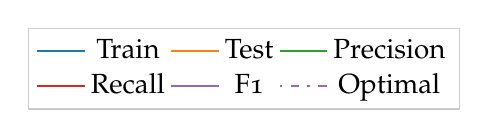
\begin{tikzpicture}

\definecolor{color0}{rgb}{0.12156862745098,0.466666666666667,0.705882352941177}
\definecolor{color1}{rgb}{1,0.498039215686275,0.0549019607843137}
\definecolor{color2}{rgb}{0.172549019607843,0.627450980392157,0.172549019607843}
\definecolor{color3}{rgb}{0.83921568627451,0.152941176470588,0.156862745098039}
\definecolor{color4}{rgb}{0.580392156862745,0.403921568627451,0.741176470588235}
\begin{axis}[%
 hide axis,
 xmin=10,
 xmax=50,
 ymin=0,
 ymax=0.4,
 legend columns=3,
 legend style={
   fill opacity=1,
   draw opacity=1,
   text opacity=1,
   align=center,
   anchor=north,
   draw=white!80!black
 },
 ]
 \addlegendimage{semithick, color0}
 \addlegendentry{Train};
 \addlegendimage{semithick, color1}
 \addlegendentry{Test};
 \addlegendimage{semithick, color2}
 \addlegendentry{Precision};
 \addlegendimage{semithick, color3}
 \addlegendentry{Recall};
 \addlegendimage{semithick, color4}
 \addlegendentry{F1};
 \addlegendimage{semithick, color4, dash pattern=on 1pt off 3pt on 3pt off 3pt}
 \addlegendentry{Optimal};
 \end{axis}

\end{tikzpicture}

  \end{subfigure}
\par\bigskip
  \begin{subfigure}[b]{0.5\textwidth}
    \input{figures/optimizing-parameters/02-augmented-ferrenti-approach-176-LOG.tex}
    \caption{}
    \label{fig:q2-LOG}
  \end{subfigure}%
  \hfill
  \begin{subfigure}[b]{0.5\textwidth}
    \input{figures/optimizing-parameters/02-augmented-ferrenti-approach-176-DT.tex}
    \caption{}
    \label{fig:q2-DT}
  \end{subfigure}

  \begin{subfigure}[b]{0.5\textwidth}
    \input{figures/optimizing-parameters/02-augmented-ferrenti-approach-176-RF.tex}
    \caption{}
    \label{fig:q2-RF}
  \end{subfigure}%
  \hfill
  \begin{subfigure}[b]{0.5\textwidth}
    \input{figures/optimizing-parameters/02-augmented-ferrenti-approach-176-GB.tex}
    \caption{}
    \label{fig:q2-GB}
  \end{subfigure}
  \caption{{Four figures displaying hyperparameter search for the augmented Ferrenti approach. The best estimator is visualized for all hyperparameters as a function of principal components during a grid search with a $5\times5$ stratified cross-validation, and the dotted lines mark the optimal hyperparameter-combination. Train stands for normal training accuracy, while test is the balanced accuracy on the test set. Precision, recall, and F$1$ scores are based on the test set. The number of principal components that explain the $95 \ \%$ accumulated variance is $159$, while the optimal model is found using the F$1$-score.}}
  \label{fig:02-pca}
\end{figure}

The relevant hyperparameters for the logistic regression model were the regularization strength and the maximum iterations, which were set to $0.46$ and $400$, respectively. Smaller regularization values resulted in worse scores, while increasing values did not notably alter the results. The decision trees and random forests found an optimal maximum depth of $7$, where smaller values resulted in low precision but high recall. Therefore, the choice was made to facilitate a compromise between precision and recall. For gradient boosting, we find the optimal maximum depth as $4$ due to a decline in overall metrics for increasing depth except for training accuracy, which could potentially result in overfitting.


The interpretation of feature importance for the augmented Ferrenti approach is substantially more difficult than in the Ferrenti approach. We find for logistic regression and decision trees that no feature is different than any other in the cross-validation due to a large variety of accuracy. However, we find that random forests and gradient boosting experience the fifth principal component as important. Similar to the Ferrenti approach, the corresponding features with the highest value for the first principal component originates the DFT band gap of the elemental solids among the elements in the composition.

\subsubsection*{Intuitive approach}

Lastly, we turn to the intuitive approach, which resulted in $404$ unsuitable and $202$ suitable candidates in the training set, which was again somewhat imbalanced. However, in contrast to the two training sets discussed above, the majority of the entries was in this case labeled as unsuitable candidates. 

The grid search for the optimal number of principal components is visualized in Figure~\ref{fig:03-pca}. Interestingly, we find that all models experience high scores for just a few principal components, where $1$ principal component earns at least $0.93$ scores for all evaluation metrics. %This information was also revealed for an earlier two-dimensional visualization of a scatter plot showing the two most important principal components in figure \ref{fig:2dscatterplotpca}, and consequently can make the models find the optimal decision boundary more easily.

Logistic regression experiences improvement of all scores for an increasing number of principal components, yet only up $5 \ \%$ in scores compared to the one-dimensional representation of one principal component. Thus, one can argue whether the increase in performance is worthwhile, considering a one-dimensional representation with just a few percentage losses of performance. However, with multiple principal components, we find the largest increase in precision, which is a sign that the one-dimensional representation tends to wrongly predict candidates as suitable when they are in fact unsuitable. The decision trees and the random forests models exhibit the best performance for just a few principal components, and experience a considerable degree of overfitting for larger values. Gradient boosting, in contrast to the case for the two Ferrenti based approaches, also experiences the best performance for a few principal components.

\begin{table}[b]
\centering
\caption{ Optimal number of principal components and the respective scores (standard deviation) for each of the four ML models logistic regression (LOG), decision trees (DT), random forests (RF) and gradient boosting (GB) in the intuitive approach, as visualized by the dash-dotted line in Figure~\ref{fig:03-pca}.}
\label{tab:03-pca}
\noindent\makebox[\textwidth]{
\begin{tabular}{M{1.0cm} M{1.0cm} M{2.0cm} M{2.0cm}M{2.0cm}M{2.0cm} }
  \hline
  \hline
   Model & PC & Mean test & Mean precision & Mean recall  & mean F1\\
  \hline
  LOG & $61$  & $0.99(0.011)$ & $0.97(0.032)$ & $0.99(0.016)$ & $0.98(0.018)$ \\
  DT & $9$    & $0.96(0.019)$ & $0.95(0.040)$ & $0.95(0.033)$ & $0.95(0.026)$ \\
  RF & $27$   & $0.98(0.020)$ & $0.97(0.033)$ & $0.97(0.031)$ & $0.97(0.026)$ \\
  GB & $13$   & $0.97(0.016)$ & $0.96(0.036)$ & $0.97(0.029)$ & $0.96(0.022)$ \\
  \hline
\end{tabular}
}
\end{table}

\begin{figure}[ht!]
  \begin{subfigure}[b]{1.0\textwidth}
    \centering
    % This file was created by tikzplotlib v0.9.8.
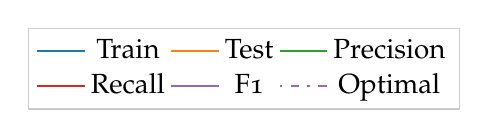
\begin{tikzpicture}

\definecolor{color0}{rgb}{0.12156862745098,0.466666666666667,0.705882352941177}
\definecolor{color1}{rgb}{1,0.498039215686275,0.0549019607843137}
\definecolor{color2}{rgb}{0.172549019607843,0.627450980392157,0.172549019607843}
\definecolor{color3}{rgb}{0.83921568627451,0.152941176470588,0.156862745098039}
\definecolor{color4}{rgb}{0.580392156862745,0.403921568627451,0.741176470588235}
\begin{axis}[%
 hide axis,
 xmin=10,
 xmax=50,
 ymin=0,
 ymax=0.4,
 legend columns=3,
 legend style={
   fill opacity=1,
   draw opacity=1,
   text opacity=1,
   align=center,
   anchor=north,
   draw=white!80!black
 },
 ]
 \addlegendimage{semithick, color0}
 \addlegendentry{Train};
 \addlegendimage{semithick, color1}
 \addlegendentry{Test};
 \addlegendimage{semithick, color2}
 \addlegendentry{Precision};
 \addlegendimage{semithick, color3}
 \addlegendentry{Recall};
 \addlegendimage{semithick, color4}
 \addlegendentry{F1};
 \addlegendimage{semithick, color4, dash pattern=on 1pt off 3pt on 3pt off 3pt}
 \addlegendentry{Optimal};
 \end{axis}

\end{tikzpicture}

  \end{subfigure}
  \par\bigskip
  \begin{subfigure}[b]{0.5\textwidth}
    \input{figures/optimizing-parameters/03-insightful-approach-176-LOG.tex}
    \caption{}
    \label{fig:q3-LOG}
  \end{subfigure}%
  \hfill
  \begin{subfigure}[b]{0.5\textwidth}
    \input{figures/optimizing-parameters/03-insightful-approach-176-DT.tex}
    \caption{}
    \label{fig:q3-DT}
  \end{subfigure}
  \begin{subfigure}[b]{0.5\textwidth}
    \input{figures/optimizing-parameters/03-insightful-approach-176-RF.tex}
    \caption{}
    \label{fig:q3-RF}
  \end{subfigure}%
  \hfill
  \begin{subfigure}[b]{0.5\textwidth}
    \input{figures/optimizing-parameters/03-insightful-approach-176-GB.tex}
    \caption{}
    \label{fig:q3-GB}
  \end{subfigure}

  \caption{{Four figures displaying hyperparameter search for the intuitive approach. The best estimator is visualized for all hyperparameters as a function of principal components during a grid search with a $5\times5$ stratified cross-validation, and the dotted lines mark the optimal hyperparameter-combination. Train stands for normal training accuracy, while test is the balanced accuracy on the test set. Precision, recall, and F$1$-scores are based on the test set. The number of principal components that explain the $95 \ \%$ accumulated variance is $103$, while the optimal model is found using the F$1$-score.}}
  \label{fig:03-pca}
\end{figure}

The optimal hyperparameters are summarized in Table~\ref{tab:03-pca}, where all models exhibit high evaluation metrics. Importantly, we find the difference in the number of principal components as most prominent, where logistic regression finds an optimum at $61$ with the F$1$-score of $0.98$. The decision trees model uses only $9$ principal components to achieve an F$1$ score of $0.95$, while random forests needs $27$ principal components to gain an F$1$ score of $0.97$.

\begin{figure}[ht!]
  \begin{subfigure}[b]{0.5\textwidth}
    \centering
    \input{figures/feature-importance/03-insightful-approachLOG-final-2.tex}
    \label{fig:03-fi-a}
  \end{subfigure}%
  
  \begin{subfigure}[b]{0.5\textwidth}
    \centering
    \input{figures/feature-importance/03-insightful-approachDT-final-2.tex}
    \label{fig:03-fi-b}
  \end{subfigure}%
  
  \begin{subfigure}[b]{0.5\textwidth}
    \centering
    \input{figures/feature-importance/03-insightful-approachRF-final-2.tex}
    \label{fig:03-fi-c}
  \end{subfigure}%
  
  \begin{subfigure}[b]{0.5\textwidth}
    \centering
    \input{figures/feature-importance/03-insightful-approachGB-final-2.tex}
    \label{fig:03-fi-d}
  \end{subfigure}%
  
  \begin{subfigure}[b]{0.5\textwidth}
    \centering
    \input{figures/feature-importance/03-insightful-approachPC-final-2.tex}
    \label{fig:03-fi-e}
  \end{subfigure}%
  
  \caption{Five figures visualizing different parameters for the $15$ most principal components ranked in descending order by the explained variance for the intuitive approach. The panels show the logistic regression coefficients, decision trees feature importance, random forests feature importance, gradient boosting feature importance, and explained variance that is retained by including each of the eigenvectors. }
  \label{fig:03-fi}
\end{figure}

Lastly, gradient boosting performs optimally at $13$ principal components with a mean F$1$-score of $0.96$. The relevant hyperparameters were the regularization term for logistic regression, which was set to $0.021$, and the maximum number of iterations as $400$. The decision trees uses a maximum depth of $6$, where larger values increased the training accuracy but not any other metric. The maximum depth for the random forests model was set to $6$, and gradient boosting was given a value of $4$. 

The intuitive approach differs in many aspects from the Ferrenti and augmented Ferrenti approaches. Firstly, we find that the number of principal components necessary to obtain $95 \ \%$ variance is reduced to $103$ components, which is $41$ and $56$ less than the Ferrenti and augmented Ferrenti approach, respectively. Thus, the variance of the training set is found to be described with fewer principal components, indicating a simpler model.   

Secondly, we find that the first principal component is by far the most important feature for all models, as visualized in Figure~\ref{fig:03-fi}. This is part of the reason why we experience a large accuracy for only a single feature, as seen in Figure~\ref{fig:03-pca}. The first principal component's corresponding features are challenging to explain due to small variations of values, but we see it including 
%However, it differs when it comes to which top features the first principal component describes, which includes 
bond orientational parameters, coordination numbers, and the radial distribution function of a compound's crystal system.

Thirdly, the intuitive approach differs in how much explained variation is retained by the first component, which is $21 \ \%$, while it is $14 \ \%$ for the Ferrenti approach and $11 \ \%$ for the augmented Ferrenti approach. We find the difference striking considering that the approaches share the same ultimate goal, but where the training sets apparently exhibit large and significant variations. 

\begin{figure}[t]
    \centering
    (a)
    \\
    \begin{forest}
        for tree={l sep=1em, s sep=1em, anchor=center, inner sep=0.3em, fill=red!50, circle}
        [$23623$ compounds, node box, alias=bagging, above=1em
        [Logistic regression,node box,alias=a1
          [$11243$]
          [$12380$,fill=green!50,edge label={node[above=1ex,green arrow]{}}
          ]
        ]
        [Decision trees,node box,alias=a1
          [$12308$]
          [$11315$,fill=green!50,edge label={node[above=1ex,green arrow]{}}
          ]
        ]
        [Random forests,node box,alias=a1
          [$9345$]
          [$14278$,fill=green!50,edge label={node[above=1ex,green arrow]{}}
          ]
        ]
        [Gradient boosting,node box,alias=a1
          [$11835$]
          [$11788$,fill=green!50,edge label={node[above=1ex,green arrow]{}}
          ]
        ]
        ]
    \end{forest}
%\vspace*{-95mm}
    \\
    (b)
    \\
\begin{forest}
    for tree={l sep=1em, s sep=1em, anchor=center, inner sep=0.3em, fill=red!50, circle}
    [$22550$ compounds, node box, alias=bagging, above=1em
    [Logistic regression,node box,alias=a1
      [$7557$]
      [$14993$,fill=green!50,edge label={node[above=1ex,green arrow]{}}
      ]
    ]
    [Decision trees,node box,alias=a1
      [$8143$]
      [$14407$,fill=green!50,edge label={node[above=1ex,green arrow]{}}
      ]
    ]
    [Random forests,node box,alias=a1
      [$7199$]
      [$15351$,fill=green!50,edge label={node[above=1ex,green arrow]{}}
      ]
    ]
    [Gradient boosting,node box,alias=a1
      [$8762$]
      [$13788$,fill=green!50,edge label={node[above=1ex,green arrow]{}}
      ]
    ]
    ]
  \end{forest}
%\vspace*{20mm}
    \\
    (c)
    \\
 \begin{forest}
    for tree={l sep=1em, s sep=1em, anchor=center, inner sep=0.3em, fill=red!50, circle}
    [$24544$ compounds, node box, alias=bagging, above=1em
    [Logistic regression,node box,alias=a1
      [$23702$]
      [$842$,fill=green!50,edge label={node[above=1ex,green arrow]{}}
      ]
    ]
    [Decision trees,node box,alias=a1
      [$23347$]
      [$1197$,fill=green!50,edge label={node[above=1ex,green arrow]{}}
      ]
    ]
    [Random forests,node box,alias=a1
      [$24001$]
      [$543$,fill=green!50,edge label={node[above=1ex,green arrow]{}}
      ]
    ]
    [Gradient boosting,node box,alias=a1
      [$23948$]
      [$596$,fill=green!50,edge label={node[above=1ex,green arrow]{}}
      ]
    ]
    ]
  \end{forest}
\vspace*{-95mm}
\caption{Visualization of the predicted material candidates from the (a) Ferrenti, (b) augemented Ferrenti and (c) insightful approaches. The green nodes display the number of predicted suitable candidates while unsuitable ones are marked in red.}
\label{fig:predictions}
\end{figure}



\section*{Supplementary results} 

\subsection*{Prediction statistics}

Figure~\ref{fig:predictions} provides a visualization of the number of predicted material candidates from the (a) Ferrenti, (b) augmented Ferrenti and (c) intuitive approaches. Suitable and unsuitable candidates are marked in green and red, respectively. We observe that the number of predicted suitable candidates is similar for the Ferrenti and augmented Ferrenti approaches, albeit higher in the case of the latter, for all four ML models, while the intuitive approach results in a substantially narrower selection of contender materials. Note that the confidence cut-off was set to $0.5$. 

For the Ferrenti approach, logistic regression finds a total of $12.380$ suitable candidates, while decision trees is the most conservative with $11.315$. random forests has the most optimistic estimate with $14.278$, while gradient boosting finds $11.835$ suitable candidates. The four ML models agree on $6804$ suitable candidates, however, many of the materials
are predicted with a confidence similar to that of a coin-flip.
If we were to raise the minimum bar of a prediction to
$0.7$, the models would only agree on $3000$ suitable candidates

The perhaps more liberal augmented Ferrenti approach yields the largest number of predicted candidates with $14.993$, $14.407$, $15.351$ and $13.788$ for logistic regression, decision trees, random forests, and gradient boosting, respectively. Due to the less stringent restrictions compared to the Ferrenti approach, we find the large amount of $9227$ entries that the four models agree on.

The four models predict radically fewer suitable candidates for the intuitive approach as compared to the two former approaches, where only $842$, $1197$, $543$, and $596$ materials are predicted suitable by logistic regression, decision trees, random forests, and gradient boosting, respectively. The large majority of the unsuitable candidates are predicted with high probability except for the random forests model due to the ensemble of trees. All models, however, agree on $214$ suitable candidates. 

\subsection*{Predicted materials}

Table~\ref{tab:03-probability-candidates} displays the $66$ predicted candidate materials that all four machine learning models, using the training set derived in the intuitive approach, agreed on with a confidence cut-off set to $0.75$. All band gaps are taken from the Materials Project database as calculated using DFT and the PBE functional. Note that materials can appear several times  on  the  list due  to  different  structures of the same composition. The  list  contains $5$ elementary (unary), $46$  binary and  $15$ ternary compounds. 

\begin{center}
\begin{longtable}{M{3.5cm} M{6.5cm} M{2.0cm}}
\caption{The $66$ predicted candidates that all models in the intuitive approach agreed on to a cut-off of $0.75$. All band gaps were taken from the Materials Project (MP) database, and materials can appear several times in the list due to different structures. The list contains $5$ elementary (unary), $46$ binary and $15$ ternary compounds.}
\label{tab:03-probability-candidates}  
\\ \hline
Compound formula & MP ID & Band gap from MP (eV) \\
\hline
  Ge & mp-137 & 0.87\\
  CdTe & mp-406 & 1.22\\
  HgSe & mp-820 & 0.12\\
  GeTe & mp-938 & 0.82\\
  MgTe & mp-1039 & 2.36\\
  CdSe & mp-1070 & 0.55\\
  GaSb & mp-1156 & 0.36\\
  BP & mp-1479 & 1.46\\
  MoSe$_2$ & mp-1634 & 1.41\\
  BN & mp-1639 & 4.64\\
  YbTe & mp-1779 & 1.52\\
  SnS & mp-1876 & 0.95\\
  SnTe & mp-1883 & 0.66\\
  GeTe & mp-2612 & 0.61\\
  AlSb & mp-2624 & 1.26\\
  CdSe & mp-2691 & 0.50\\
  SnSe & mp-2693 & 0.82\\
  CdSnAs$_2$ & mp-3829 & 0.30\\
  GaCuTe$_2$ & mp-3839 & 0.55\\
  ZnGeAs$_2$ & mp-4008 & 0.56\\
  ZnGeP$_2$ & mp-4524 & 1.20\\
  GaAgTe$_2$ & mp-4899 & 0.19\\
  CdSnP$_2$ & mp-5213 & 0.67\\
  GaCuS$_2$ & mp-5238 & 0.70\\
  SnS & mp-10013 & 0.23\\
  BAs & mp-10044 & 1.25\\
  GeSe & mp-10759 & 0.44\\
  MgSe & mp-10760 & 1.97\\
  CdTe & mp-12779 & 0.61\\
  MgSe & mp-13031 & 2.54\\
  MgTe & mp-13033 & 2.31\\
  TePb & mp-19717 & 1.05\\
  InAs & mp-20305 & 0.30\\
  InP & mp-20351 & 0.46\\
  InAgSe$_2$ & mp-20554 & 0.36\\
  InN & mp-22205 & 0.47\\
  AgI & mp-22894 & 1.39\\
  CuI & mp-22895 & 1.17\\
  CuBr & mp-22913 & 0.48\\
  CuCl & mp-22914 & 0.80\\
  AgI & mp-22919 & 1.00\\
  AgI & mp-22925 & 1.72\\
  Br & mp-23154 & 1.32\\
  TlI & mp-23197 & 2.25\\
  AgBr & mp-23231 & 0.79\\
  BC$_2$N & mp-30148 & 2.10\\
  CuI & mp-569346 & 1.21\\
  Hg & mp-569360 & 0.22\\
  Ga$_2$Os & mp-570875 & 0.66\\
  BC$_2$N & mp-629458 & 1.84\\
  InP & mp-966800 & 0.51\\
  GeC & mp-1002164 & 1.84\\
  TlP & mp-1007776 & 0.12\\
  BC$_2$N & mp-1008523 & 1.64\\
  BP & mp-1008559 & 1.07\\
  OsC & mp-1009540 & 0.17\\
  SiSn & mp-1009813 & 0.41\\
  ZnCdSe$_2$ & mp-1017534 & 1.85\\
  MgSe & mp-1018040 & 2.57\\
  AlSb & mp-1018100 & 0.91\\
  AlBi & mp-1018132 & 0.30\\
  Ge & mp-1067619 & 0.791\\
  Ga$_2$Ru & mp-1072429 & 0.12\\
  ZnCd$_3$Se$_4$ & mp-1078597 & 1.72\\
  BC$_2$N & mp-1079201 & 1.17\\
  Ge & mp-1198022 & 0.67\\
  \hline
\end{longtable}
\end{center}


Table~\ref{tab:04-probability-candidates} displays the $47$ predicted candidates that all four machine learning models and all three approaches agreed upon. 
%To 0.5 cutoff 
The list contains $8$ elemental, $29$ binary, and $10$ tertiary compounds.

\begin{center}
\begin{longtable}{M{3.5cm} M{6.5cm} M{2.0cm}}
\caption{A table displaying the $46$? predicted candidates that all models and all approaches agree on.}
\label{tab:03-probability-candidates}  
\hline
Compound formula & MP ID & Band gap from MP (eV) \\
\hline
  P & mp-157 & 7.47\\
  SiRu & mp-189 & 0.63\\
  BN & mp-344 & 0.41\\
  HgSe & mp-820 & 3.96\\
  FeSi & mp-871 & 2.06\\
  MgTe & mp-1039 & 6.62\\
  CdSe & mp-1070 & 3.91\\
  BP & mp-1479 & 2.89\\
  CdSe & mp-2691 & 2.40\\
  ZnSiAs$_2$ & mp-3595 & 1.57\\
  ZnGeAs$_2$ & mp-4008 & 1.52\\
  CdSnP$_2$ & mp-5213 & 0.95\\
  Si$_2$Mo & mp-8938 & 0.66\\
  BAs & mp-10044 & 0.61\\
  GeSe & mp-10759 & 1.26\\
  N$_2$ & mp-12103 & 0.50\\
  BeSiN$_2$ & mp-15704 & 0.82\\
  InP & mp-20351 & 0.30\\
  InN & mp-22205 & 0.55\\
  AgCl & mp-22922 & 0.56\\
  I & mp-23153 & 1.20\\
  Br & mp-23154 & 0.19\\
  TlI & mp-23197 & 0.67\\
  AgBr & mp-23231 & 0.70\\
  H$_2$ & mp-23907 & 0.23\\
  Ge$_3$As$_4$ & mp-569600 & 1.25\\
  TlCl & mp-569639 & 0.44\\
  Sn$_3$As$_4$ & mp-570377 & 1.97\\
  H$_2$ & mp-634659 & 0.61\\
  N$_2$ & mp-672234 & 2.54\\
  TiFe$_2$Ge & mp-866375 & 2.31\\
  InP & mp-966800 & 1.05\\
  GeC & mp-1002164 & 0.30\\
  B$_2$AsP & mp-1008528 & 0.46\\
  BP & mp-1008559 & 0.36\\
  BeSiAs$_2$ & mp-1009087 & 0.47\\
  OsC & mp-1009540 & 1.39\\
  ScP & mp-1009746 & 1.17\\
  SiSn & mp-1009813 & 0.48\\
  SnC & mp-1009820 & 0.80\\
  AlBi & mp-1018132 & 1.00\\
  Al$_3$BN$_4$ & mp-1019380 & 1.72\\
  GeRu & mp-1025397 & 1.32\\
  PbS & mp-1057015 & 2.25\\
  Ge & mp-1067619 & 0.79\\
  ZnCd$_3$S$_4$ & mp-1078780 & 2.10\\
  Ga$_4$BiAs$_3$ & mp-1079228 & 1.21\\
  \hline
\end{longtable}
\end{center}


\subsection*{Feature analysis}
%Or important features for QT 
Figure~\ref{fig:histograms_supp} displays the number of predicted suitable materials for all approaches (all ML models in an approach agree to a $0.75$ confidence level) as a function of the (a) covalent radius of the elements in the composition, (b) maximum packing efficiency, and standard deviation of the radial distribution function (RDF) with center at (c) $2.0$ and (d) $3.0$. The corresponding figure in the main text shows the standard deviation of the RDF with Gaussian center at $1.0$. Several observations can be made based on the histograms. Panels (e) chemical environment site fingerprint, (f) crystal fingerprint and (g) OP site fingerprint are related to bond orientational parameters, while (h) shows the material band gaps referenced to the normalized mean of the entire data set.  

Firstly, we find that the covalent radii of the materials (see Fig.~\ref{fig:histograms_supp}a) distribute with two peaks in the data in all approaches. The maxima are slightly shifted towards the right for the empirical approach compared to the two others but otherwise the data distributions are similar. The trend of two data peaks is repeated for the maximum packing efficiency (see Fig.~\ref{fig:histograms_supp}b) but is much more prominent for the empirical approach. This indicates that the material density, or in other words the bond length, is an important parameter for QT suitability.  


%histograms 
\begin{figure}[h!]
    \centering
    \includegraphics[width=0.4\textwidth]{figures/histograms/new/ElementProperty_MagpieData range CovalentRadius_count_075.pdf}
    \includegraphics[width=0.4\textwidth]{figures/histograms/new/MaximumPackingEfficiency_max packing efficiency_count_075.pdf}
    \includegraphics[width=0.4\textwidth]{figures/histograms/new/GeneralizedRDF_std_dev Gaussian center=2.0 width=1.0_count_075.pdf}
    \includegraphics[width=0.4\textwidth]{figures/histograms/new/GeneralizedRDF_std_dev Gaussian center=3.0 width=1.0_count_075.pdf}
    \includegraphics[width=0.4\textwidth]{figures/histograms/new/ChemEnvSiteFingerprint_GaussianSymmFuncstd_dev G2_20.0_count_075.pdf}
    \includegraphics[width=0.4\textwidth]{figures/histograms/new/CrystalNNFingerprint_mean tetrahedral CN_4_count_075.pdf} 
    \includegraphics[width=0.4\textwidth]{figures/histograms/new/OPSiteFingerprint_mean tetrahedral CN_4_count_075.pdf} 
    \includegraphics[width=0.4\textwidth]{figures/histograms/new/MP_Eg_normalized_databackgrund_075.pdf} 
    \caption{Histograms of predicted suitable materials as a function of the (a) covalent radius, (b) maximum packing efficiency, and standard deviation of the radial distribution function with center at (c) $2.0$ and (d) $3.0$. Panels (e) chemical environment site fingerprint, (f) crystal fingerprint and (g) OP site fingerprint are related to bond orientational parameters, while (h) shows the band gap referenced to the normalized mean of the entire data set. The total number of predicted materials is  $6804$ for the Ferrenti approach, $9227$ for the extended Ferrenti approach, and $214$ for the empirical approach. The Ferrenti and extended Ferrenti approaches refer to the left y-axis and the empirical approach to the right. All panels were taken for a $0.75$ cut-off. }
    \label{fig:histograms_supp}
\end{figure} 

\newpage 
 
\bibliography{apssamp}% Produces the bibliography via BibTeX.

\end{document}

